\subsection{Crystalline Rock Samples}
\Authors{TU Freiberg}
\todo[inline]{[TUBAF](): Introduction to URL Reiche Zeche}

\begin{figure}[!ht]
\begin{center}
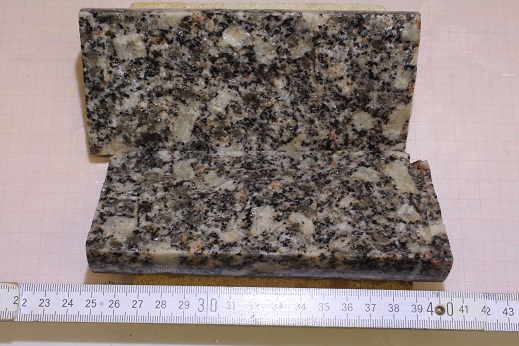
\includegraphics[width=0.5\textwidth]{./figures/ExpRockGranite.JPG}
\end{center}
\caption{Granite sample}
\label{fig:RockGranite}
\end{figure}

\begin{figure}[!ht]
\begin{center}
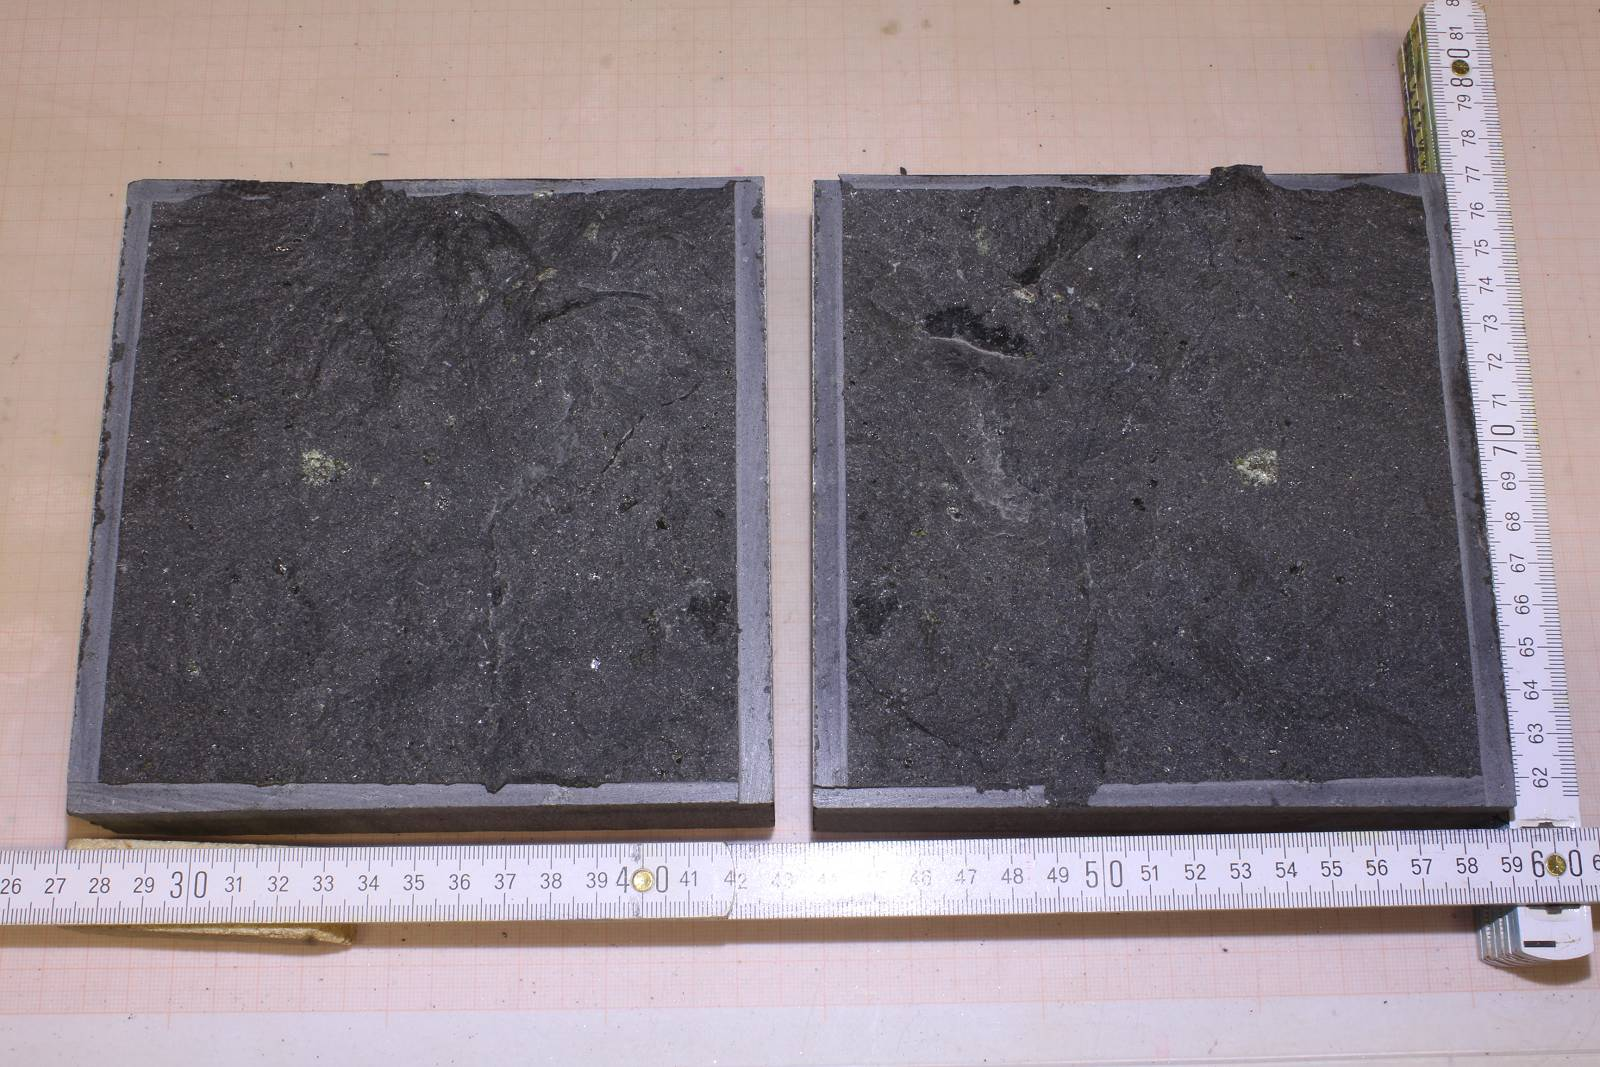
\includegraphics[width=0.5\textwidth]{./figures/ExpRockBasalt.jpg}
\end{center}
\caption{Basalt sample}
\label{fig:RockBasalt}
\end{figure}

Two different crystalline rock types are used. Granite is a coarse-grained intrusive igneous rock. The grains are on the millimetre to centimetre scale, see Fig. \ref{fig:RockGranite}. The typical main minerals of granites are quartz, feldspar and plagioclase.\\
Basalt is an fine-grained extrusive igneous rock. It is rich of plagioclase. See Fig. \ref{fig:RockBasalt}.\\
Lab tests to evaluate basic rock parameters of the intact rock material like elastic constants, compressive strength, cohesion or friction angle have been conducted. The values of the granite and basalt used in the experiments can be found in table \ref{table:MEX7_rockParam}.\\
\begin{table}[!ht]
\begin{center}
\begin{tabular}{l c r r r}
variable & symbol & granite & basalt & unit\\
\hline
density & $\rho$ & $2.59$ &3.06 &$\text{g}/\text{cm}^3$\\
compressive strength & $u_c$ & $120.54$&272.92 &$\text{MPa}   $\\
tensile strength & $u_t$ & $7.02$&16.61 &$ \text{MPa}   $\\
%static elastic modulus & $E_s$ & $50.00$& &$ \text{GPa}   $\\
elastic modulus & $E$ & $49.75$&105.46 &$ \text{GPa}   $\\
Poisson's ratio & $\nu$ & 0.26 & 0.26  & -\\
fracture toughness & $K_I$ & $0.95$& 2.61 &$\text{MPa}\cdot\text{m}^{0.5}$\\
friction angle (Mohr) & $\Phi$ &  $52.5$& 44 &$^\circ$\\
cohesion & $c$ &  $22.5$& 25.00  &$ \text{MPa}   $\\
basic friction angle &$\Phi_b$ &30 & 31.2 & $^\circ$\\
\end{tabular}
\caption{Rock parameters of granite and basalt used in the direct shear tests.}
\label{table:MEX7_rockParam}
\end{center}
\end{table}